% Options for packages loaded elsewhere
\PassOptionsToPackage{unicode}{hyperref}
\PassOptionsToPackage{hyphens}{url}
%
\documentclass[
  ignorenonframetext,
]{beamer}
\usepackage{pgfpages}
\setbeamertemplate{caption}[numbered]
\setbeamertemplate{caption label separator}{: }
\setbeamercolor{caption name}{fg=normal text.fg}
\beamertemplatenavigationsymbolsempty
% Prevent slide breaks in the middle of a paragraph
\widowpenalties 1 10000
\raggedbottom
\setbeamertemplate{part page}{
  \centering
  \begin{beamercolorbox}[sep=16pt,center]{part title}
    \usebeamerfont{part title}\insertpart\par
  \end{beamercolorbox}
}
\setbeamertemplate{section page}{
  \centering
  \begin{beamercolorbox}[sep=12pt,center]{part title}
    \usebeamerfont{section title}\insertsection\par
  \end{beamercolorbox}
}
\setbeamertemplate{subsection page}{
  \centering
  \begin{beamercolorbox}[sep=8pt,center]{part title}
    \usebeamerfont{subsection title}\insertsubsection\par
  \end{beamercolorbox}
}
\AtBeginPart{
  \frame{\partpage}
}
\AtBeginSection{
  \ifbibliography
  \else
    \frame{\sectionpage}
  \fi
}
\AtBeginSubsection{
  \frame{\subsectionpage}
}
\usepackage{amsmath,amssymb}
\usepackage{lmodern}
\usepackage{iftex}
\ifPDFTeX
  \usepackage[T1]{fontenc}
  \usepackage[utf8]{inputenc}
  \usepackage{textcomp} % provide euro and other symbols
\else % if luatex or xetex
  \usepackage{unicode-math}
  \defaultfontfeatures{Scale=MatchLowercase}
  \defaultfontfeatures[\rmfamily]{Ligatures=TeX,Scale=1}
\fi
% Use upquote if available, for straight quotes in verbatim environments
\IfFileExists{upquote.sty}{\usepackage{upquote}}{}
\IfFileExists{microtype.sty}{% use microtype if available
  \usepackage[]{microtype}
  \UseMicrotypeSet[protrusion]{basicmath} % disable protrusion for tt fonts
}{}
\makeatletter
\@ifundefined{KOMAClassName}{% if non-KOMA class
  \IfFileExists{parskip.sty}{%
    \usepackage{parskip}
  }{% else
    \setlength{\parindent}{0pt}
    \setlength{\parskip}{6pt plus 2pt minus 1pt}}
}{% if KOMA class
  \KOMAoptions{parskip=half}}
\makeatother
\usepackage{xcolor}
\newif\ifbibliography
\usepackage{color}
\usepackage{fancyvrb}
\newcommand{\VerbBar}{|}
\newcommand{\VERB}{\Verb[commandchars=\\\{\}]}
\DefineVerbatimEnvironment{Highlighting}{Verbatim}{commandchars=\\\{\}}
% Add ',fontsize=\small' for more characters per line
\usepackage{framed}
\definecolor{shadecolor}{RGB}{248,248,248}
\newenvironment{Shaded}{\begin{snugshade}}{\end{snugshade}}
\newcommand{\AlertTok}[1]{\textcolor[rgb]{0.94,0.16,0.16}{#1}}
\newcommand{\AnnotationTok}[1]{\textcolor[rgb]{0.56,0.35,0.01}{\textbf{\textit{#1}}}}
\newcommand{\AttributeTok}[1]{\textcolor[rgb]{0.77,0.63,0.00}{#1}}
\newcommand{\BaseNTok}[1]{\textcolor[rgb]{0.00,0.00,0.81}{#1}}
\newcommand{\BuiltInTok}[1]{#1}
\newcommand{\CharTok}[1]{\textcolor[rgb]{0.31,0.60,0.02}{#1}}
\newcommand{\CommentTok}[1]{\textcolor[rgb]{0.56,0.35,0.01}{\textit{#1}}}
\newcommand{\CommentVarTok}[1]{\textcolor[rgb]{0.56,0.35,0.01}{\textbf{\textit{#1}}}}
\newcommand{\ConstantTok}[1]{\textcolor[rgb]{0.00,0.00,0.00}{#1}}
\newcommand{\ControlFlowTok}[1]{\textcolor[rgb]{0.13,0.29,0.53}{\textbf{#1}}}
\newcommand{\DataTypeTok}[1]{\textcolor[rgb]{0.13,0.29,0.53}{#1}}
\newcommand{\DecValTok}[1]{\textcolor[rgb]{0.00,0.00,0.81}{#1}}
\newcommand{\DocumentationTok}[1]{\textcolor[rgb]{0.56,0.35,0.01}{\textbf{\textit{#1}}}}
\newcommand{\ErrorTok}[1]{\textcolor[rgb]{0.64,0.00,0.00}{\textbf{#1}}}
\newcommand{\ExtensionTok}[1]{#1}
\newcommand{\FloatTok}[1]{\textcolor[rgb]{0.00,0.00,0.81}{#1}}
\newcommand{\FunctionTok}[1]{\textcolor[rgb]{0.00,0.00,0.00}{#1}}
\newcommand{\ImportTok}[1]{#1}
\newcommand{\InformationTok}[1]{\textcolor[rgb]{0.56,0.35,0.01}{\textbf{\textit{#1}}}}
\newcommand{\KeywordTok}[1]{\textcolor[rgb]{0.13,0.29,0.53}{\textbf{#1}}}
\newcommand{\NormalTok}[1]{#1}
\newcommand{\OperatorTok}[1]{\textcolor[rgb]{0.81,0.36,0.00}{\textbf{#1}}}
\newcommand{\OtherTok}[1]{\textcolor[rgb]{0.56,0.35,0.01}{#1}}
\newcommand{\PreprocessorTok}[1]{\textcolor[rgb]{0.56,0.35,0.01}{\textit{#1}}}
\newcommand{\RegionMarkerTok}[1]{#1}
\newcommand{\SpecialCharTok}[1]{\textcolor[rgb]{0.00,0.00,0.00}{#1}}
\newcommand{\SpecialStringTok}[1]{\textcolor[rgb]{0.31,0.60,0.02}{#1}}
\newcommand{\StringTok}[1]{\textcolor[rgb]{0.31,0.60,0.02}{#1}}
\newcommand{\VariableTok}[1]{\textcolor[rgb]{0.00,0.00,0.00}{#1}}
\newcommand{\VerbatimStringTok}[1]{\textcolor[rgb]{0.31,0.60,0.02}{#1}}
\newcommand{\WarningTok}[1]{\textcolor[rgb]{0.56,0.35,0.01}{\textbf{\textit{#1}}}}
\usepackage{graphicx}
\makeatletter
\def\maxwidth{\ifdim\Gin@nat@width>\linewidth\linewidth\else\Gin@nat@width\fi}
\def\maxheight{\ifdim\Gin@nat@height>\textheight\textheight\else\Gin@nat@height\fi}
\makeatother
% Scale images if necessary, so that they will not overflow the page
% margins by default, and it is still possible to overwrite the defaults
% using explicit options in \includegraphics[width, height, ...]{}
\setkeys{Gin}{width=\maxwidth,height=\maxheight,keepaspectratio}
% Set default figure placement to htbp
\makeatletter
\def\fps@figure{htbp}
\makeatother
\setlength{\emergencystretch}{3em} % prevent overfull lines
\providecommand{\tightlist}{%
  \setlength{\itemsep}{0pt}\setlength{\parskip}{0pt}}
\setcounter{secnumdepth}{-\maxdimen} % remove section numbering
\ifLuaTeX
  \usepackage{selnolig}  % disable illegal ligatures
\fi
\IfFileExists{bookmark.sty}{\usepackage{bookmark}}{\usepackage{hyperref}}
\IfFileExists{xurl.sty}{\usepackage{xurl}}{} % add URL line breaks if available
\urlstyle{same} % disable monospaced font for URLs
\hypersetup{
  pdftitle={Scenario tree method},
  pdfauthor={Eleftherios Meletis \& Aurélien Madouasse},
  hidelinks,
  pdfcreator={LaTeX via pandoc}}

\title{Scenario tree method}
\author{Eleftherios Meletis \& Aurélien Madouasse}
\date{2022-09-14}

\begin{document}
\frame{\titlepage}

\begin{frame}{Scenario tree method - Introduction}
\protect\hypertarget{scenario-tree-method---introduction}{}
Reference quantitative method to estimate the probability of freedom
from infection from complex surveillance systems

Answers to:

\begin{itemize}
\tightlist
\item
  If infection was present at the design prevalence, what would be the
  probability of the surveillance system detecting at least 1 case?
  \textbf{Surveillance sensitivity}
\item
  Given that no cases have been detected, what is the probability that
  the true prevalence of infection is lower than the design prevalence?
  \textbf{Probability of freedom from infection}
\end{itemize}

Principle: A surveillance system is represented as a tree with different
components
\end{frame}

\begin{frame}{Scenario tree method - Simple Example}
\protect\hypertarget{scenario-tree-method---simple-example}{}
We will go through a simple example that will help understand

\begin{enumerate}
\item Scenario tree notation 
\item Scenario tree calculations
\end{enumerate}

\begin{itemize}
\tightlist
\item
  Objective: Estimation of the probability of freedom from Bovine Viral
  Diarrhea virus (BVDV) in country A (simple example) and Country B
  (complex example)
\end{itemize}
\end{frame}

\begin{frame}{}
\protect\hypertarget{section}{}
The following figure shows the structure of the surveillance system for
country A.

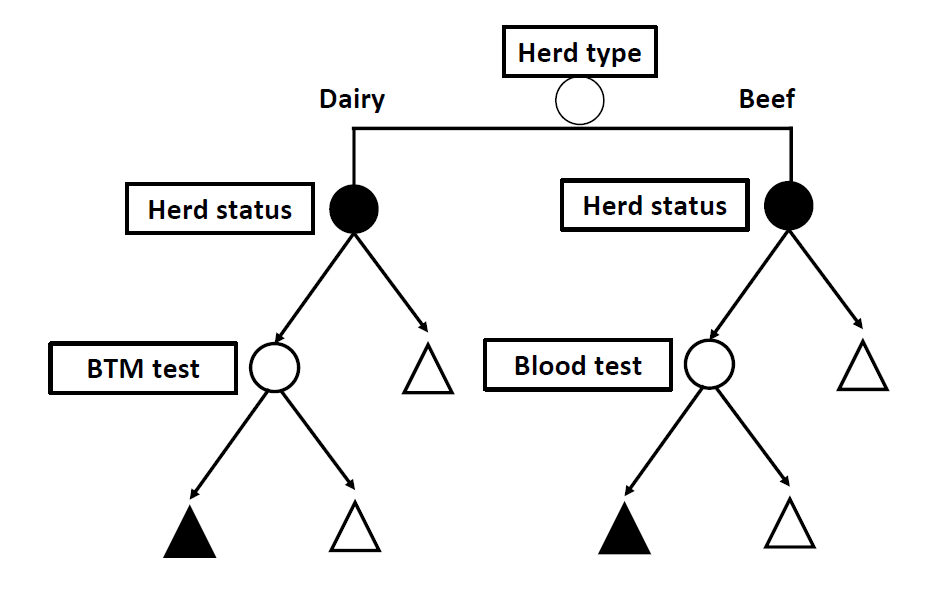
\includegraphics{figs/simple_scenario_tree.png}
\end{frame}

\begin{frame}{Scenario tree method - Figure Explained}
\protect\hypertarget{scenario-tree-method---figure-explained}{}
The surveillance system is split, given the herd type, to dairy and beef
cattle.

We assume that the design prevalence is the same for both dairy and beef
cattle.

Given the herd type a different diagnostic method to detect infection is
applied.

\begin{itemize}
\item Dairy - Bulk Tank Milk
\item Beef - Blood  sample [e.g., serum ELISA]
\end{itemize}
\end{frame}

\begin{frame}{Scenario tree notation}
\protect\hypertarget{scenario-tree-notation}{}
\begin{itemize}
\tightlist
\item
  Herd type - (Risk) Category node
\item
  Herd status - Infection node
\item
  BTM test / Blood test - Detection nodes
\end{itemize}

\vspace{1cm}

\begin{itemize}
\tightlist
\item
  (Risk) Category node(s) - represent(s) (risk) factors dividing the
  surveillance system population into subsets with different
  probabilities of being infected
\item
  Infection node - represent the infection status, branch probabilities
  derived from design prevalence
\item
  Detection node(s) - represent(s) the detection of infection,
  associated with test characteristics
\end{itemize}
\end{frame}

\begin{frame}{Scenario tree calculations (I)}
\protect\hypertarget{scenario-tree-calculations-i}{}
\begin{block}{Constraints}
\protect\hypertarget{constraints}{}
\begin{enumerate}
\item All final results from the surveillance system are consistent with country or zone freedom from infection
\item Specificity (Sp) of the surveillance system is 1 
\end{enumerate}
\end{block}
\end{frame}

\begin{frame}{Scenario tree calculations (II)}
\protect\hypertarget{scenario-tree-calculations-ii}{}
\begin{itemize}
\item
  Complex Surveillance systems can have more than one detection nodes
  (see example later)
\item
  Units with a positive test outcome at the first detection node are
  retested (with a ``better'' method / more ``specific'' method). The
  final result has to be negative.
\item
  The process of repeated testing (sequential testing)

  \begin{enumerate}
  \item Reduces the probability of a false-positive output in the surveillance system (SS) (Sp of SS = 1)
  \item If a true-positive unit is detected then the country's/zone's claim of freedom from infection is no longer valid and the method is no longer applicable
  \end{enumerate}
\end{itemize}

\begin{block}{Extra Assumption}
\protect\hypertarget{extra-assumption}{}
Often the Sps of the individual methods applied are considered 100\%
\end{block}
\end{frame}

\begin{frame}[fragile]{Simple Example - R code}
\protect\hypertarget{simple-example---r-code}{}
\begin{block}{Input parameters}
\protect\hypertarget{input-parameters}{}
\begin{itemize}
\tightlist
\item
  Design prevalence
\item
  Test characteristics of BTM and Blood test
\item
  Number of herds tested, per herd type
\end{itemize}

\begin{Shaded}
\begin{Highlighting}[]
\CommentTok{\# Design prevalence}
\NormalTok{p\_design }\OtherTok{=} \FloatTok{0.02}
\CommentTok{\#Test characteristics}
\CommentTok{\# BTM test}
\NormalTok{Se\_BTM }\OtherTok{=} \FloatTok{0.98}
\NormalTok{Sp\_BTM }\OtherTok{=} \DecValTok{1}
\CommentTok{\# Blood test}
\NormalTok{Se\_Blood }\OtherTok{=} \FloatTok{0.95}
\NormalTok{Sp\_Blood }\OtherTok{=} \DecValTok{1}
\CommentTok{\# Number of herds tested, per herd type}
\CommentTok{\# Different scenario given sample size}
\NormalTok{n\_dairy }\OtherTok{=} \FunctionTok{seq}\NormalTok{(}\DecValTok{10}\NormalTok{,}\DecValTok{400}\NormalTok{,}\DecValTok{20}\NormalTok{)}
\NormalTok{n\_beef }\OtherTok{=} \FunctionTok{seq}\NormalTok{(}\DecValTok{10}\NormalTok{,}\DecValTok{600}\NormalTok{,}\DecValTok{10}\NormalTok{)}
\end{Highlighting}
\end{Shaded}
\end{block}
\end{frame}

\begin{frame}[fragile]{Estimate Surveillance component sensitivity
(SCSe)}
\protect\hypertarget{estimate-surveillance-component-sensitivity-scse}{}
\begin{block}{Surveillance component sensitivity (SCSe)}
  \begin{equation}
          SCSe = 1 - (1 - p^**Se)^n
  \end{equation}

  \begin{equation}
          OverallSSe = 1 - prod_{i=1}^{n}(1 - SCSe_n)
  \end{equation}
\end{block}

\begin{Shaded}
\begin{Highlighting}[]
\NormalTok{CSE\_dairy }\OtherTok{=} \DecValTok{1} \SpecialCharTok{{-}}\NormalTok{ (}\DecValTok{1}\SpecialCharTok{{-}}\NormalTok{(p\_design}\SpecialCharTok{*}\NormalTok{Se\_BTM))}\SpecialCharTok{\^{}}\NormalTok{n\_dairy}
\NormalTok{CSE\_beef }\OtherTok{=} \DecValTok{1} \SpecialCharTok{{-}}\NormalTok{ (}\DecValTok{1}\SpecialCharTok{{-}}\NormalTok{(p\_design}\SpecialCharTok{*}\NormalTok{Se\_Blood))}\SpecialCharTok{\^{}}\NormalTok{n\_beef}

\NormalTok{Overall\_SSE }\OtherTok{=} \DecValTok{1} \SpecialCharTok{{-}}\NormalTok{ (}\DecValTok{1}\SpecialCharTok{{-}}\NormalTok{CSE\_dairy)}\SpecialCharTok{*}\NormalTok{(}\DecValTok{1}\SpecialCharTok{{-}}\NormalTok{CSE\_beef)}
\end{Highlighting}
\end{Shaded}

Compare efficacies of the two SCs - Sensitivity ratio

\emph{Critical value is 1}

\begin{Shaded}
\begin{Highlighting}[]
\NormalTok{Sensitivity\_ratio }\OtherTok{=}\NormalTok{ CSE\_dairy}\SpecialCharTok{/}\NormalTok{CSE\_beef}
\end{Highlighting}
\end{Shaded}
\end{frame}

\begin{frame}[fragile]{Estimate probability of freedom from infection}
\protect\hypertarget{estimate-probability-of-freedom-from-infection}{}
\begin{block}{Pr(freedom)}
  Pr(freedom) = Pr(D- | S-) = Negative Predictive Value
  \begin{equation}
  \begin{aligned}
  \begin{split}
  &Pr_f = Pr(D^- | S^-) = \frac{Pr(S^- | D^-) Pr(D^-))}{Pr(S^-)} =\\
  &\frac{Pr(S^- | D^-) Pr(D^-) )}{Pr(S^- | D^-) Pr(D^-) + Pr(S^-|D^+)*Pr(D^+)}\\ 
  &= \frac{Sp_S * (1-p^*)}{Sp_S * (1-p^*) + (1 - Se_S)*p^*}\\
  \end{split}
  \end{aligned}
  \end{equation}

\end{block}

\begin{block}{Assuming that Sp of SS = 1 then}
  \begin{equation}
        Pr_f = Pr(D^- | S^-) = \frac{(1-p^*)}{(1-p^*) + (1 - Se_S)*P^*}
  \end{equation}

\end{block}

\begin{Shaded}
\begin{Highlighting}[]
\NormalTok{P\_freedom}\OtherTok{=}\NormalTok{(}\DecValTok{1}\SpecialCharTok{{-}}\NormalTok{p\_design)}\SpecialCharTok{/}
\NormalTok{  ((}\DecValTok{1}\SpecialCharTok{{-}}\NormalTok{p\_design)}\SpecialCharTok{+}\NormalTok{p\_design}\SpecialCharTok{*}\NormalTok{(}\DecValTok{1}\SpecialCharTok{{-}}\NormalTok{Overall\_SSE))}
\end{Highlighting}
\end{Shaded}
\end{frame}

\begin{frame}{Another example - Homework Exercise}
\protect\hypertarget{another-example---homework-exercise}{}
\begin{block}{Introducing the Adjusted risk}
\protect\hypertarget{introducing-the-adjusted-risk}{}
Suppose the following scenario for a surveillance system for BVDV

\begin{itemize}
\tightlist
\item
  Country B has 2 regions
\item
  In each region herds are divided given herd type to beef and dairy
  cattle
\item
  Dairy cattle tested by BTM - if positive retested \textbar{} Beef
  cattle tested with ELISA - if positive retested
\end{itemize}

Region 2 is sharing borders with a country that is known to be
BVDV-positive - higher risk

\begin{itemize}
\tightlist
\item
  Relative\_risk(region\_2) = 4*Relative\_risk(region\_1) = 4
\item
  Relative\_risk(region\_1) = 1
\end{itemize}

80\% of the herds belong to Region 1

\begin{itemize}
\tightlist
\item
  40\% beef cattle \textbar{} 60\% dairy cattle
\end{itemize}

20\% of the herds belong to Region 2

\begin{itemize}
\tightlist
\item
  40\% beef cattle \textbar{} 60\% dairy cattle
\end{itemize}

Design prevalence = 0.02
\end{block}
\end{frame}

\begin{frame}{Scenario tree - Figure}
\protect\hypertarget{scenario-tree---figure}{}
Construct the scenario tree for country B, with the information provided
above. Use scenario tree for country A, as a starting point.

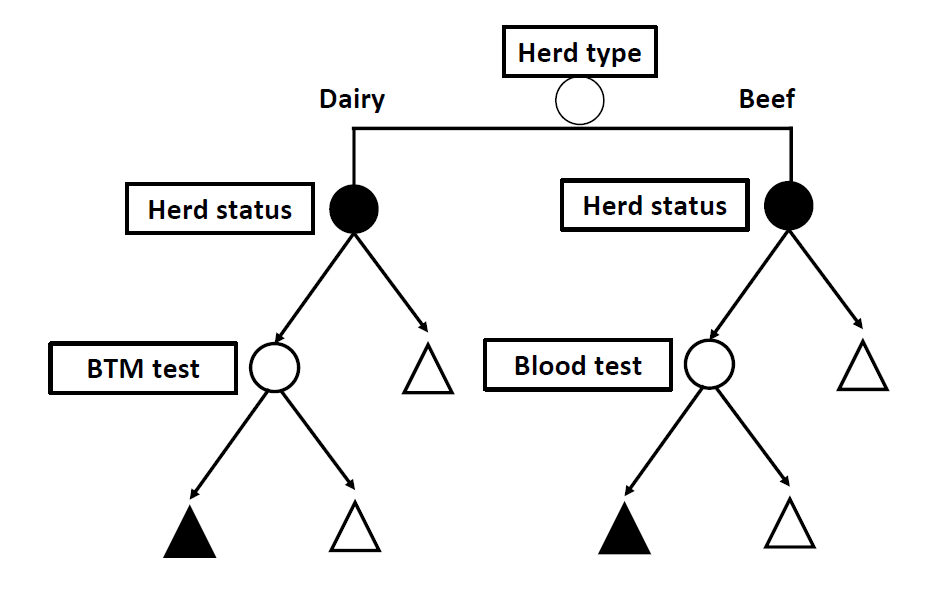
\includegraphics{figs/simple_scenario_tree.png}
\end{frame}

\begin{frame}{Scenario tree - Figure}
\protect\hypertarget{scenario-tree---figure-1}{}
\begin{block}{DONE??}
\protect\hypertarget{done}{}
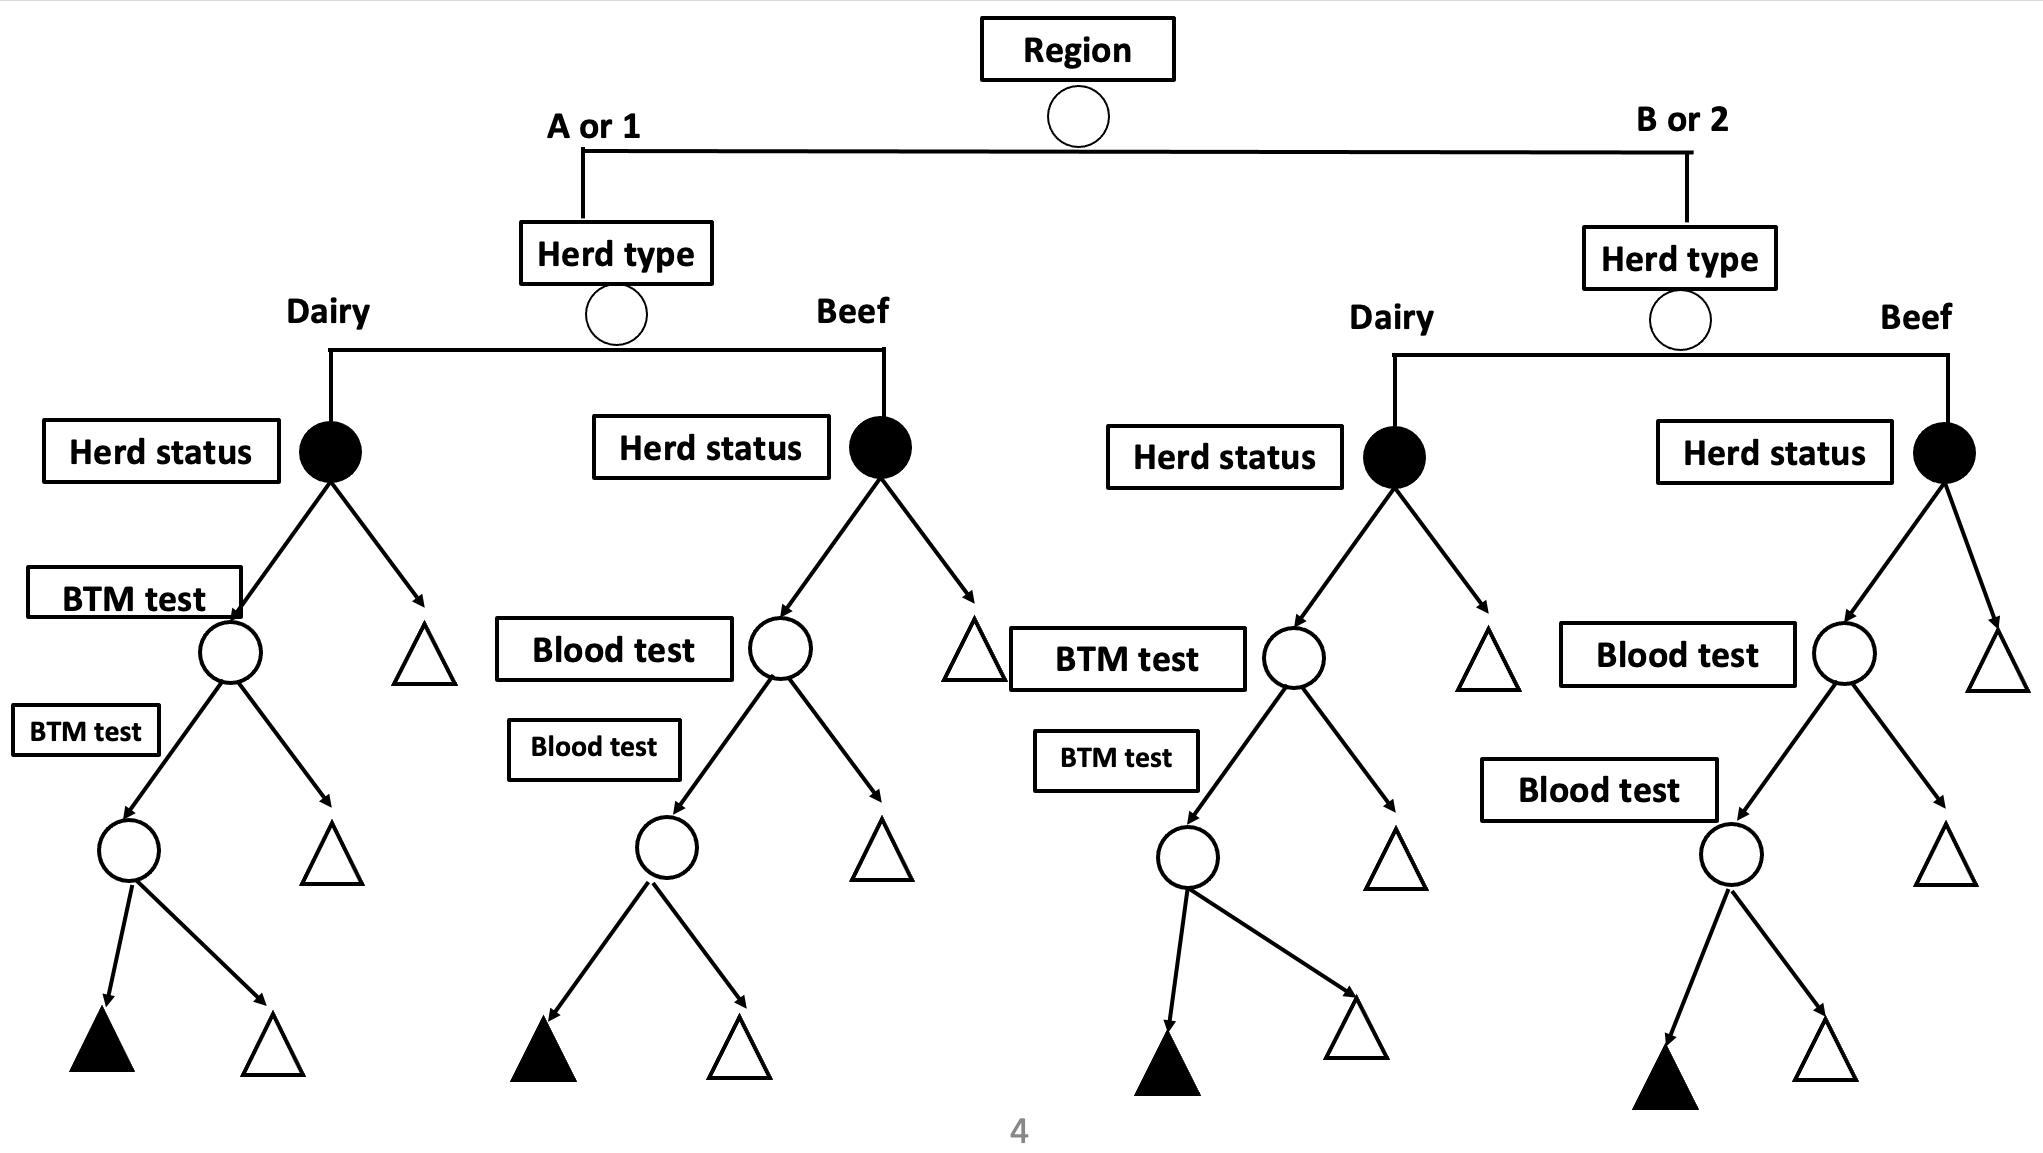
\includegraphics{figs/second_example_scenario_tree.png}
\end{block}
\end{frame}

\begin{frame}{Scenario tree - Figure Explained}
\protect\hypertarget{scenario-tree---figure-explained}{}
\begin{itemize}
\item
  Now region is a risk category node!
\item
  The available relative risks have to be adjusted given the proportion
  of the population in each branch of the node.
\end{itemize}

The output value is known as \textbf{Adjusted Risk}.
\end{frame}

\begin{frame}{Calculation of Adjusted Risk}
\protect\hypertarget{calculation-of-adjusted-risk}{}
\begin{block}{Key Points}
\protect\hypertarget{key-points}{}
\begin{block}{Ratio of adjusted risks must remain the same as the original relative risk}
  \begin{equation}
      AR_1/AR_2 = RR_1/RR_2
  \end{equation}
\end{block}

\begin{block}{The average risk across the population is equal to 1}
  \begin{equation}
      AR_1 * Pr(Region_1) + AR_2 * Pr(Region_2) = 1
  \end{equation}
\end{block}
\end{block}
\end{frame}

\begin{frame}[fragile]{Second Example - R code}
\protect\hypertarget{second-example---r-code}{}
AR\_1 = 1/(Pr(Region\_1) + RR\_2 * Pr(Region\_2))

AR\_2 = RR\_2 * AR\_1

\begin{Shaded}
\begin{Highlighting}[]
\NormalTok{RR\_1 }\OtherTok{=} \DecValTok{1}
\NormalTok{RR\_2 }\OtherTok{=} \DecValTok{4}
\NormalTok{P\_region\_1 }\OtherTok{=} \FloatTok{0.8}
\NormalTok{P\_region\_2 }\OtherTok{=} \FloatTok{0.2}
\end{Highlighting}
\end{Shaded}

\begin{Shaded}
\begin{Highlighting}[]
\NormalTok{AR\_1 }\OtherTok{=} \DecValTok{1}\SpecialCharTok{/}\NormalTok{(P\_region\_1 }\SpecialCharTok{+}\NormalTok{ RR\_2}\SpecialCharTok{*}\NormalTok{P\_region\_2)}
\NormalTok{AR\_2 }\OtherTok{=}\NormalTok{ RR\_2 }\SpecialCharTok{*}\NormalTok{ AR\_1}
\end{Highlighting}
\end{Shaded}
\end{frame}

\begin{frame}[fragile]{Effective probability of infection}
\protect\hypertarget{effective-probability-of-infection}{}
!!! As a last step we have to adjust for the design prevalence

The output defined as Effective Probability of infection (EPI) is equal
to

\begin{block}{Formula}
  \begin{equation}
         EPI = AR*p^*
  \end{equation}
\end{block}

\begin{Shaded}
\begin{Highlighting}[]
\NormalTok{p\_design }\OtherTok{=} \FloatTok{0.02}
\NormalTok{EPI\_1 }\OtherTok{=}\NormalTok{ AR\_1}\SpecialCharTok{*}\NormalTok{p\_design}
\NormalTok{EPI\_2 }\OtherTok{=}\NormalTok{ AR\_2}\SpecialCharTok{*}\NormalTok{p\_design}
\end{Highlighting}
\end{Shaded}
\end{frame}

\begin{frame}[fragile]{Repeated testing}
\protect\hypertarget{repeated-testing}{}
As pointed out if a unit tests positive in the first round of testing
then it is retested with the same test.

Assuming independence between tests the overall sensitivity of the
sequential testing is the product of the individual sensitivities

\begin{Shaded}
\begin{Highlighting}[]
\CommentTok{\#Test characteristics}
\CommentTok{\# BTM test}
\NormalTok{Se\_BTM }\OtherTok{=} \FloatTok{0.98}
\NormalTok{Sp\_BTM }\OtherTok{=} \DecValTok{1}
\CommentTok{\# Blood test}
\NormalTok{Se\_Blood }\OtherTok{=} \FloatTok{0.95}
\NormalTok{Sp\_Blood }\OtherTok{=} \DecValTok{1}

\NormalTok{Seq\_Dairy }\OtherTok{=}\NormalTok{ Se\_BTM}\SpecialCharTok{\^{}}\DecValTok{2}
\NormalTok{Seq\_Blood }\OtherTok{=}\NormalTok{ Se\_Blood}\SpecialCharTok{\^{}}\DecValTok{2}
\end{Highlighting}
\end{Shaded}
\end{frame}

\begin{frame}[fragile]{Sample Size}
\protect\hypertarget{sample-size}{}
\begin{Shaded}
\begin{Highlighting}[]
\CommentTok{\# Total herds sampled in Country B}
\NormalTok{n\_total }\OtherTok{=} \FunctionTok{seq}\NormalTok{(}\DecValTok{1000}\NormalTok{, }\DecValTok{100000}\NormalTok{, }\DecValTok{10}\NormalTok{)}
\CommentTok{\# 80\% Region 1 | 20\% Region 2}
\CommentTok{\# 40\% beef | 60\% dairy}
\NormalTok{n\_1\_dairy }\OtherTok{=} \FloatTok{0.8} \SpecialCharTok{*} \FloatTok{0.6} \SpecialCharTok{*}\NormalTok{ n\_total}
\NormalTok{n\_1\_beef }\OtherTok{=} \FloatTok{0.8} \SpecialCharTok{*} \FloatTok{0.4} \SpecialCharTok{*}\NormalTok{ n\_total}
\NormalTok{n\_2\_dairy }\OtherTok{=} \FloatTok{0.2} \SpecialCharTok{*} \FloatTok{0.6} \SpecialCharTok{*}\NormalTok{ n\_total}
\NormalTok{n\_2\_dairy }\OtherTok{=} \FloatTok{0.2} \SpecialCharTok{*} \FloatTok{0.4} \SpecialCharTok{*}\NormalTok{ n\_total}
\end{Highlighting}
\end{Shaded}
\end{frame}

\begin{frame}[fragile]{Surveillance Sensitivity}
\protect\hypertarget{surveillance-sensitivity}{}
We are now ready to estimate the component and overall surveillance
sensitivities

\begin{Shaded}
\begin{Highlighting}[]
\CommentTok{\# d: dairy | b: beef}
\NormalTok{CSE\_A\_d }\OtherTok{=} \DecValTok{1} \SpecialCharTok{{-}}\NormalTok{ (}\DecValTok{1}\SpecialCharTok{{-}}\NormalTok{(EPI\_1}\SpecialCharTok{*}\NormalTok{Seq\_Dairy))}\SpecialCharTok{\^{}}\NormalTok{n\_1\_dairy}
\NormalTok{CSE\_A\_b }\OtherTok{=} \DecValTok{1} \SpecialCharTok{{-}}\NormalTok{ (}\DecValTok{1}\SpecialCharTok{{-}}\NormalTok{(EPI\_1}\SpecialCharTok{*}\NormalTok{Seq\_Blood))}\SpecialCharTok{\^{}}\NormalTok{n\_1\_beef}

\NormalTok{CSE\_B\_d }\OtherTok{=} \DecValTok{1} \SpecialCharTok{{-}}\NormalTok{ (}\DecValTok{1}\SpecialCharTok{{-}}\NormalTok{(EPI\_2}\SpecialCharTok{*}\NormalTok{Seq\_Dairy))}\SpecialCharTok{\^{}}\NormalTok{n\_2\_dairy}
\NormalTok{CSE\_B\_b }\OtherTok{=} \DecValTok{1} \SpecialCharTok{{-}}\NormalTok{ (}\DecValTok{1}\SpecialCharTok{{-}}\NormalTok{(EPI\_2}\SpecialCharTok{*}\NormalTok{Seq\_Blood))}\SpecialCharTok{\^{}}\NormalTok{n\_2\_dairy}

\NormalTok{Overall\_SSE }\OtherTok{=} \DecValTok{1} \SpecialCharTok{{-}} 
\NormalTok{  (}\DecValTok{1}\SpecialCharTok{{-}}\NormalTok{CSE\_A\_d)}\SpecialCharTok{*}\NormalTok{(}\DecValTok{1}\SpecialCharTok{{-}}\NormalTok{CSE\_A\_b)}\SpecialCharTok{*}\NormalTok{(}\DecValTok{1}\SpecialCharTok{{-}}\NormalTok{CSE\_B\_d)}\SpecialCharTok{*}\NormalTok{(}\DecValTok{1} \SpecialCharTok{{-}}\NormalTok{ CSE\_B\_b)}
\end{Highlighting}
\end{Shaded}
\end{frame}

\begin{frame}[fragile]{Estimate probability of freedom from infection}
\protect\hypertarget{estimate-probability-of-freedom-from-infection-1}{}
\begin{Shaded}
\begin{Highlighting}[]
\NormalTok{P\_freedom}\OtherTok{=}\NormalTok{(}\DecValTok{1}\SpecialCharTok{{-}}\NormalTok{p\_design)}\SpecialCharTok{/}
\NormalTok{  ((}\DecValTok{1}\SpecialCharTok{{-}}\NormalTok{p\_design)}\SpecialCharTok{+}\NormalTok{p\_design}\SpecialCharTok{*}\NormalTok{(}\DecValTok{1}\SpecialCharTok{{-}}\NormalTok{Overall\_SSE))}
\end{Highlighting}
\end{Shaded}
\end{frame}

\begin{frame}{Conclusions}
\protect\hypertarget{conclusions}{}
\begin{itemize}
\tightlist
\item
  Questions???
\end{itemize}

Suggested literature

\begin{itemize}
\tightlist
\item
  Martin et al, (2007) Demonstrating freedom from disease using multiple
  complex data sources
\item
  Norström et al, (2014) Estimation of the probability of freedom from
  BVDV in Norway using scenario tree modelling
\end{itemize}
\end{frame}

\end{document}
